% Download-page OS glyph: macOS — a generic whole apple (leaf + stem) on a grey
% badge. A plain fruit drawing, deliberately NOT the bitten-apple brand mark.
\documentclass[tikz,border=1mm]{standalone}
\usetikzlibrary{arrows.meta,calc}
\definecolor{macbg}{HTML}{8A8F98}
\definecolor{leaf}{HTML}{7CC243}
\definecolor{stem}{HTML}{6B4A2B}
\begin{document}
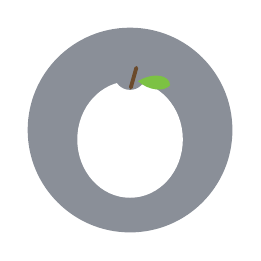
\begin{tikzpicture}[line cap=round, line join=round, x=1mm,y=1mm]
  \fill[macbg] (0,0) circle (13);
  % rounded apple body
  \fill[white] (0,-1.2) ellipse (6.7 and 7.4);
  % carve a small top-centre dimple (same colour as the badge)
  \fill[macbg] (0,7.1) circle (2.0);
  % stem rising from the dimple
  \draw[stem, line width=1.4pt] (0.1,5.4) -- (0.8,7.9);
  % leaf beside the stem
  \fill[leaf] (1.0,6.2) .. controls (3.0,7.4) and (5.0,7.0) .. (5.1,5.7)
                        .. controls (4.3,4.8) and (2.4,5.0) .. (1.0,6.2) -- cycle;
\end{tikzpicture}
\end{document}
